% Sources: Neso videos (one-time pad, rail fence, row-column transposition; notes5.md), college Lecture 5 slides 54-55,
% Stallings 2.2-2.3, Forouzan 3.2. Every number recomputed by script (scratchpad/r3/verify.py).
\providecommand{\railfence}[1]{%
  \foreach \l/\r [count=\i] in {#1}{\node[font=\small] (rf\i) at (\i*0.5,-\r*0.6) {\l};}}

\section{One-Time Pad \hot}\label{sec:otp}
\asked{Mid-sem 2025--26 Q1 (8 marks): OTP-Vigen\`ere with key stream 9 0 1 7 23 15 21 14 11 11 2 8 9 (Stallings 2.x). Part (b), finding a key that maps the ciphertext to another plaintext, is exactly why an OTP is unbreakable: every plaintext of the same length is possible.}

\subsection{How it grew out of the earlier ciphers}
Every substitution cipher so far was broken through the same flaw: the key is reused, so some regularity of the plaintext survives into the ciphertext. A monoalphabetic cipher applies one fixed substitution to the whole message, so the letter frequencies of English pass straight through. Vigen\`ere rotates through $m$ substitutions, so once $m$ is known the ciphertext splits into $m$ interleaved Caesar ciphers (\S\ref{sec:classextra} shows how the Kasiski test finds $m$). The autokey cipher removes the period by continuing the key with the plaintext itself, but then the key is English text and carries English statistics. Vernam's cipher (1918) works on bits with a long key stream punched on paper tape, but the tape was a loop, so the key eventually repeated and a long enough message could be broken.

Shannon's study of secrecy showed what the key must look like for \emph{no} regularity to survive: each plaintext symbol must be encrypted with a key symbol chosen \textbf{at random from the whole key domain}, independently of every other symbol. Even the weak additive cipher becomes perfect under this rule. It is broken easily because the same shift is used for every letter; but if the first letter is shifted by 04, the second by 02, the third by 21, and each shift is drawn at random from $00, 01, \dots, 25$, then nothing links one ciphertext letter to another or to the plaintext. This is the \textbf{one-time pad} (OTP), the last substitution technique of the course and an improvement to the Vernam cipher (Stallings credits the improvement to Joseph Mauborgne; Forouzan's slides credit Vernam).

\begin{center}\small
\begin{tabularx}{\textwidth}{@{}l X X@{}}
\toprule
Cipher & Key & What goes wrong\\
\midrule
Vigen\`ere & short keyword, \textbf{repeated} & repeats every $m$ letters $\Rightarrow$ split into Caesar ciphers\\
Autokey & keyword + plaintext & key is English $\Rightarrow$ has English letter frequencies\\
Vernam & long key stream (paper tape) & tape loops, so the key \textbf{eventually repeats}\\
\textbf{One-time pad} & \textbf{truly random}, \textbf{same length} as message, \textbf{used once} & nothing to exploit\\
\bottomrule
\end{tabularx}
\end{center}

\subsection{Definition and mechanism}
In a one-time pad the key is a \textbf{truly random} sequence that is \textbf{as long as the message}, so it never has to be repeated. The key is used to encrypt and decrypt \textbf{a single message} and is then \textbf{discarded}; every new message needs a new random key of its own length. The encryption rule itself is unchanged from Vigen\`ere (letters) or Vernam (bits): only the key is different. Stallings calls the result ``the ultimate in security'', because such a scheme is unbreakable.

\begin{mustknow}[: one-time pad]
\textbf{Key}: truly random, same length as the message, used once, then destroyed.\\[2pt]
\textbf{Letters}: $C_i = (P_i + K_i) \bmod 26$, \;$P_i = (C_i - K_i) \bmod 26$. \qquad \textbf{Bits}: $C_i = P_i \oplus K_i$, \;$P_i = C_i \oplus K_i$.\\[2pt]
\textbf{Perfect secrecy}: $\Pr[M \mid C] = \Pr[M]$; the ciphertext reveals nothing about the plaintext. The OTP is the \emph{only} cipher with this property (key at least as long as the message is necessary).\\[2pt]
\textbf{Two difficulties}: (1) making large quantities of random keys; (2) key distribution and protection.
\end{mustknow}

Decryption recovers the plaintext because the key cancels: $(P_i + K_i) - K_i \equiv P_i \pmod{26}$, and $(P_i \oplus K_i) \oplus K_i = P_i \oplus 0 = P_i$, since XOR of a bit with itself is 0. The receiver therefore needs exactly the same key, in the same order, aligned with the same letter positions; this requirement is the source of all the practical difficulties discussed below.

\subsection{Example 1: letters}
Plaintext \ttx{attackatdawn}, random key \ttx{qvhzmxkbplwe} (12 key letters for 12 plaintext letters). Each letter is shifted by its own key value, and four sums pass 25 and wrap:
\begin{center}\small\setlength{\tabcolsep}{4.5pt}
\begin{tabular}{@{}l*{12}{c}@{}}
\toprule
Plain & a&t&t&a&c&k&a&t&d&a&w&n\\
$P$ & 0&19&19&0&2&10&0&19&3&0&22&13\\
Key & q&v&h&z&m&x&k&b&p&l&w&e\\
$K$ & 16&21&7&25&12&23&10&1&15&11&22&4\\
$P+K$ & 16&\hl{40}&\hl{26}&25&14&\hl{33}&10&20&18&11&\hl{44}&17\\
$\bmod 26$ & 16&14&0&25&14&7&10&20&18&11&18&17\\
Cipher & \textbf{Q}&\textbf{O}&\textbf{A}&\textbf{Z}&\textbf{O}&\textbf{H}&\textbf{K}&\textbf{U}&\textbf{S}&\textbf{L}&\textbf{S}&\textbf{R}\\
\bottomrule
\end{tabular}
\end{center}
Ciphertext \textbf{\ttx{QOAZOHKUSLSR}}. The receiver computes $(C - K) \bmod 26$ letter by letter to get \ttx{attackatdawn} back, then destroys the key. The two \ttx{t}'s of \ttx{att} became \ttx{O} and \ttx{A}, and the two \ttx{S}'s of the ciphertext came from different letters (\ttx{d} and \ttx{w}): equal letters do not produce equal letters, and equal ciphertext letters do not mean equal plaintext letters.

\subsection{Example 2: bits}
``HI'' in 8-bit ASCII, XORed with a random 16-bit key. Each ciphertext bit is 1 exactly where the plaintext bit and the key bit differ:
\begin{center}\small\ttfamily
\begin{tabular}{@{}r@{\quad}l@{\quad}l@{}}
\rmfamily Plaintext (H, I) & 01001000 & 01001001\\
\rmfamily Key & 10110101 & 01101100\\
\midrule
\rmfamily Ciphertext $P\oplus K$ & 11111101 & 00100101\\
\rmfamily $C \oplus K$ & 01001000 & 01001001 \rmfamily\;= ``HI'' again\\
\end{tabular}
\end{center}

\subsection{Why it cannot be broken}
The one-time pad produces random output that has \textbf{no statistical relationship to the plaintext}. Since the ciphertext contains no information whatsoever about the plaintext, there is simply no way to break the code, and the security of the scheme comes \textbf{entirely from the randomness of the key}. This can be seen at three levels.

\textbf{One letter.} Suppose the attacker sees the ciphertext letter \ttx{Q} ($= 16$). Every plaintext letter could have produced it, each with exactly one key letter, namely $K = (16 - P) \bmod 26$:
\begin{center}\small\setlength{\tabcolsep}{5pt}
\begin{tabular}{@{}l*{7}{c}@{}}
\toprule
If the plaintext was & a & b & c & d & e & \dots & z\\
then the key was & q & p & o & n & m & \dots & r\\
\bottomrule
\end{tabular}
\end{center}
Since the key letter was drawn at random, all 26 cases are \textbf{equally likely}, and seeing \ttx{Q} tells the attacker nothing. The same argument shows that the ciphertext letters themselves are uniformly distributed: $\Pr[C_i = c] = \sum_p \Pr[P_i = p] \cdot \Pr[K_i = c - p] = \sum_p \Pr[P_i = p] \cdot \tfrac{1}{26} = \tfrac{1}{26}$, whatever the plaintext statistics. The ciphertext has a flat frequency histogram (no peak for \ttx{e} to aim at), and since the key never repeats, the Kasiski and index-of-coincidence tests of \S\ref{sec:classextra} find nothing.

\textbf{The whole message.} For a message of $n$ letters there are $26^n$ keys, exactly as many as there are $n$-letter strings, and every string is the decryption of the ciphertext under exactly one key. The same ciphertext therefore decrypts to anything of the same length:
\begin{center}\small
\begin{tabular}{@{}lll@{}}
\toprule
Ciphertext & Key tried & Result\\
\midrule
\ttx{QOAZOHKUSLSR} & \ttx{qvhzmxkbplwe} & \textbf{attack at dawn}\\
\ttx{QOAZOHKUSLSR} & \ttx{zkhikhruztku} & \textbf{retreat at six}\\
\ttx{KXFUDM} & \ttx{kemubc} & \textbf{attack}\\
\ttx{KXFUDM} & \ttx{htaqqj} & \textbf{defend}\\
\bottomrule
\end{tabular}
\end{center}
A brute-force search produces \emph{every} meaningful message of that length, with nothing to say which one was sent. Compare the Caesar cipher, where only one of the 25 tries makes sense (GERMANY): there the key space is far smaller than the message space, so wrong keys give gibberish and the right one stands out.

\subsection{Perfect secrecy: the derivation}
\textbf{Definition (Shannon, 1949).} A cipher has \textbf{perfect secrecy} if, for every plaintext $M$ and every ciphertext $C$ that can occur,
\[
\Pr[M \mid C] = \Pr[M].
\]
$\Pr[M]$ is what the attacker believes about the message before interception (for example, that ``no attack today'' is the usual message), and $\Pr[M \mid C]$ is what she believes after seeing $C$. Equality means the ciphertext changes nothing: \imp{given a ciphertext from a perfectly secure cipher, absolutely nothing is revealed about the plaintext.}

\textbf{The one-time pad meets the definition.} Fix any plaintext $M$ and ciphertext $C$ of length $n$. Exactly one key maps $M$ to $C$, namely $K = C - M \pmod{26}$ letter by letter (or $K = C \oplus M$ for bits). Every key is equally likely, with probability $1/26^n$, so
\[
\Pr[C \mid M] = \Pr[K = C - M] = \frac{1}{26^n}\quad\text{for every } M .
\]
Averaging over the messages, $\Pr[C] = \sum_{M} \Pr[M]\Pr[C \mid M] = \frac{1}{26^n}\sum_M \Pr[M] = \frac{1}{26^n}$. Bayes' rule then gives
\[
\Pr[M \mid C] = \frac{\Pr[C \mid M]\,\Pr[M]}{\Pr[C]} = \frac{(1/26^n)\,\Pr[M]}{1/26^n} = \Pr[M].
\]
In words: every key is equally likely, and for each candidate plaintext exactly one key turns it into the observed $C$, so $C$ ``points'' equally strongly to every plaintext, and the attacker's probabilities stay where they were. For a one-bit pad with $\Pr[M = 0] = 0.9$: $\Pr[C = 1] = 0.9 \cdot 0.5 + 0.1 \cdot 0.5 = 0.5$, and $\Pr[M = 0 \mid C = 1] = 0.5 \cdot 0.9 / 0.5 = 0.9$; Eve's best guess after interception is exactly her guess before it.

\textbf{Why the key must be as long as the message.} Suppose there were fewer keys than possible messages. Decrypting a given $C$ under all keys yields at most as many candidate plaintexts as there are keys, so some message $M$ with $\Pr[M] > 0$ is not among them and has $\Pr[M \mid C] = 0$: the ciphertext has ruled it out, and secrecy is not perfect. For example, a Caesar shift used for a two-letter message cannot turn \ttx{aa} into \ttx{AB}, because one shift maps equal letters to equal letters; seeing \ttx{AB} eliminates \ttx{aa}, \ttx{bb}, \dots. Hence perfect secrecy needs at least as many keys as messages, i.e.\ at least as much random key as message. This is Shannon's bound, and it is the reason the OTP is the \textbf{only} practical cipher with perfect secrecy.

\textbf{Unconditional versus computational security.} Perfect secrecy is the \textbf{unconditionally secure} case of \S\ref{sec:schemes}: no amount of ciphertext or computing power helps, because the information is simply not there. Every other cipher in this course (DES, AES, RSA, \dots) is only \textbf{computationally} secure: it can be broken in principle, but doing so costs more time or money than the information is worth.

\begin{trap}[: what perfect secrecy does not give]
The OTP hides the \emph{content} among messages of the \emph{same length}; it does not hide the length (if Alice's answer is ``YES'' or ``NO'', a 3-letter ciphertext gives it away). It also gives no integrity: flipping a ciphertext bit flips the same plaintext bit, and Bob cannot detect it. Integrity needs a hash or MAC (\S\ref{sec:integrity}).
\end{trap}

\subsection{The rules, and what breaks if you bend them}
\textbf{Rule 1: never reuse a key (the ``two-time pad'').} Encrypt a second message \ttx{holdposition} with the \emph{same} key \ttx{qvhzmxkbplwe}; the result is $C_2 = $ \ttx{XJSCBLCJITKR}. Subtracting the two ciphertexts cancels the key,
\[
C_1 - C_2 = (P_1 + K) - (P_2 + K) = P_1 - P_2 \pmod{26},
\]
and indeed both differences equal \ttx{TFIXNWILKSIA}. What remains is two English texts combined with each other, which has strong structure (common words, frequent letters) that the attacker can attack without knowing any key. Worse, if the attacker knows or guesses $P_1$ (``attack at dawn'' is a stock phrase), she recovers the key $K = C_1 - P_1 = $ \ttx{qvhzmxkbplwe} and then $P_2 = C_2 - K = $ \textbf{hold position}. With bits the same cancellation is $C_1 \oplus C_2 = P_1 \oplus P_2$. Historically, Soviet pads that were reused in the 1940s were partly read by the US VENONA project for exactly this reason.

\textbf{Rule 2: the key must be truly random.} If the key is text taken from a book (a \textbf{running key}), it has English letter frequencies and can be attacked like the autokey. If it is generated by a formula from a short seed, the cipher is really a stream cipher: at best \emph{computationally} secure, never perfect, because the number of possible key streams is only the number of seeds.

\textbf{Rule 3: the key must be at least as long as the message.} A shorter key has to repeat, and then the cipher is back to Vigen\`ere or Vernam with their weaknesses; the derivation above shows that perfect secrecy is then impossible.

\textbf{Known plaintext does not hurt a correctly used OTP.} If the attacker learns one plaintext and its ciphertext, she gets $K = C - P$, but only for that message, and that key is never used again. For every other cipher a known pair helps break future traffic (\S\ref{sec:classextra}); here it is worthless.

\subsection{Two fundamental difficulties}
In theory the one-time pad is the end of the story; in practice it has two fundamental difficulties.
\begin{enumerate}[leftmargin=1.5em]
  \item \imp{The practical problem of making large quantities of random keys.} Every message needs fresh random key material of the same size, so a system carrying a lot of traffic needs millions of truly random characters on a regular basis. Pseudorandom generators do not qualify (Rule 2), and good physical sources of randomness are slow.
  \item \imp{Even more daunting is the problem of key distribution and protection.} For every message, sender and receiver must hold an identical key of the same length, delivered and stored securely, and destroyed after use. If a secure channel able to carry that much key existed, the message could simply be sent over it instead.
\end{enumerate}
The second point is softened by \emph{timing}: the key can be carried in advance, by a trusted courier, at a moment and by a route the parties choose, after which the messages can travel over any insecure channel. The slide's example is a president who sends a trusted envoy with a random key to another president before sending a completely secret message. This is why Forouzan calls the OTP ``a perfect cipher, but almost impossible to implement commercially''.

\textbf{Advantages.} Perfect secrecy: no attack, however much ciphertext or computing power the attacker has, can extract information about the plaintext. Encryption and decryption are trivial additions or XORs. \textbf{Disadvantages.} The key is as long as all the traffic ever sent, must be truly random, must reach the receiver securely in advance and must never be reused; it gives no integrity. Because of these difficulties, \imp{the one-time pad is of limited utility, and is useful primarily for low-bandwidth channels requiring very high security} (diplomatic and military links).

\subsection{Exam-format one-time-pad numerical}
\begin{worked}[: Stallings 2.x, mid-sem 2025--26 Q1]
\textbf{Q.} This problem uses a one-time pad version of the Vigen\`ere cipher: each plaintext letter is shifted by the next number of the key stream \ttx{9 0 1 7 23 15 21 14 11 11 2 8 9}. (a) Encrypt \ttx{sendmoremoney}. (b) Using the ciphertext from (a), find a key stream that makes it decrypt to \ttx{cashnotneeded}. (8 marks)

\textbf{(a)} $C_i = (P_i + K_i) \bmod 26$, letters numbered from $a = 0$:
\begin{center}\small\setlength{\tabcolsep}{4pt}
\begin{tabular}{@{}l*{13}{c}@{}}
\toprule
Plain & s&e&n&d&m&o&r&e&m&o&n&e&y\\
$P$ & 18&4&13&3&12&14&17&4&12&14&13&4&24\\
$K$ & 9&0&1&7&23&15&21&14&11&11&2&8&9\\
$P{+}K$ & \hl{27}&4&14&10&\hl{35}&\hl{29}&\hl{38}&18&23&25&15&12&\hl{33}\\
mod 26 & 1&4&14&10&9&3&12&18&23&25&15&12&7\\
Cipher & \textbf{B}&\textbf{E}&\textbf{O}&\textbf{K}&\textbf{J}&\textbf{D}&\textbf{M}&\textbf{S}&\textbf{X}&\textbf{Z}&\textbf{P}&\textbf{M}&\textbf{H}\\
\bottomrule
\end{tabular}
\end{center}
Ciphertext: \textbf{\ttx{BEOKJDMSXZPMH}}.

\textbf{(b)} The key that turns $C$ into a chosen plaintext $P'$ is $K'_i = (C_i - P'_i) \bmod 26$:
\begin{center}\small\setlength{\tabcolsep}{3.6pt}
\begin{tabular}{@{}l*{13}{c}@{}}
\toprule
$C$ & B 1&E 4&O 14&K 10&J 9&D 3&M 12&S 18&X 23&Z 25&P 15&M 12&H 7\\
$P'$ & c 2&a 0&s 18&h 7&n 13&o 14&t 19&n 13&e 4&e 4&d 3&e 4&d 3\\
$C - P'$ & $-1$&4&$-4$&3&$-4$&$-11$&$-7$&5&19&21&12&8&4\\
$K'$ & \textbf{25}&\textbf{4}&\textbf{22}&\textbf{3}&\textbf{22}&\textbf{15}&\textbf{19}&\textbf{5}&\textbf{19}&\textbf{21}&\textbf{12}&\textbf{8}&\textbf{4}\\
\bottomrule
\end{tabular}
\end{center}
Key stream: \textbf{25 4 22 3 22 15 19 5 19 21 12 8 4}. Check, first letter: $(2 + 25) \bmod 26 = 1 = $ \ttx{B} \checkmark.

\textbf{Conclusion to write.} The same ciphertext decrypts to \ttx{sendmoremoney} under one key and to \ttx{cashnotneeded} under another, and both keys are equally likely random streams. An attacker who tries all keys gets every 13-letter message and cannot tell which was sent, so the one-time pad cannot be broken by brute force: it has perfect secrecy.
\end{worked}

\section{Transposition Ciphers}\label{sec:transp}
Substitution ciphers replace letters, and every one of them up to the one-time pad was attacked through the statistics of the replaced letters. A \textbf{transposition cipher} takes the opposite approach: some sort of \textbf{permutation is applied to the plaintext letters}. The letters themselves are \textbf{not replaced}; only their \textbf{positions} change, so a symbol in the first position of the plaintext may appear in the tenth position of the ciphertext. A \textbf{permutation} of $n$ positions is a rearrangement in which every position receives exactly one letter; there are $n!$ of them, and the key of a transposition cipher is a permutation or a rule (depth, column order) that generates one.

\textbf{Why transposition keeps the letter frequencies.} Every plaintext letter appears in the ciphertext exactly once, merely at another position, so the ciphertext is an \emph{anagram} of the plaintext: the two contain the same letters the same number of times, and their single-letter frequencies are identical. (Script check: the ciphertext of the Kill Corona example below has exactly the letter counts of its padded plaintext.) This gives the cryptanalyst an immediate test. If a ciphertext is unreadable but its letter counts look like normal English (\ttx{e} about 12.7\%, \ttx{t} 9.1\%, \ttx{a} 8.2\%, and \ttx{j}, \ttx{q}, \ttx{x}, \ttx{z} almost absent), the letters are genuine and only their order is scrambled: the cipher is a \textbf{transposition}. A monoalphabetic substitution shows the same \emph{shape} of histogram but on the wrong letters (the tallest bar is not \ttx{e}), and a polyalphabetic cipher flattens it. The frequency count identifies a transposition but does not break it; the attacker still has to find the order, using digram statistics (\ttx{th}, \ttx{he}, \ttx{in}, \dots) to decide which letters belong next to each other. The simplest transposition is the rail fence.

\begin{mustknow}[: transposition]
Substitution changes the \emph{letters}; transposition changes their \emph{positions}, so \textbf{letter frequencies are preserved} (a frequency count that looks like plain English means transposition).\\
Rail fence, depth $D$: zig-zag with period $2(D-1)$, read row by row. Row--column: write row by row, read column by column, \textbf{key = order of the columns}; two stages = do it again on the ciphertext.
\end{mustknow}

\subsection{Rail fence}
In the rail fence technique the plaintext is \textbf{written down as a sequence of diagonals and then read off as a sequence of rows}. The letters are written on $D$ rows (the \textbf{depth}), moving down one row per letter from row 1 to row $D$ and then back up to row 1, in a zig-zag; spaces and punctuation are dropped. The ciphertext is row 1, followed by row 2, and so on. Going down takes $D - 1$ steps and coming back takes $D - 1$ steps, so the row pattern repeats every $2(D-1)$ letters.

\textbf{Example:} ``neso academy is the best'', depth 2 (20 letters):
\begin{center}
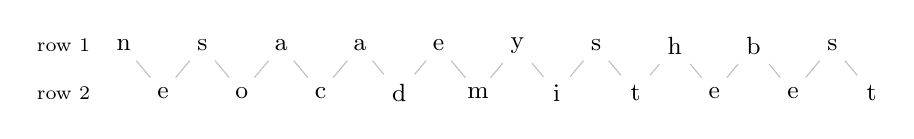
\begin{tikzpicture}
  \railfence{n/0,e/1,s/0,o/1,a/0,c/1,a/0,d/1,e/0,m/1,y/0,i/1,s/0,t/1,h/0,e/1,b/0,e/1,s/0,t/1}
  \foreach \i in {1,...,19}{\pgfmathtruncatemacro{\j}{\i+1}\draw[gray!50] (rf\i) -- (rf\j);}
  \node[font=\scriptsize,anchor=east] at (0.2,0) {row 1};
  \node[font=\scriptsize,anchor=east] at (0.2,-0.6) {row 2};
\end{tikzpicture}
\end{center}
Row 1: \ttx{NSAAEYSHBS}\quad Row 2: \ttx{EOCDMITEET}\quad $\Rightarrow$\quad \textbf{\ttx{NSAAEYSHBSEOCDMITEET}}

\textbf{Depth 3}, ``Thank you very much'' (16 letters). The path visits rows 1, 2, 3, 2, 1, 2, 3, \dots\ and repeats every $2(D-1) = 4$ letters:
\begin{center}
\begin{tikzpicture}
  \railfence{t/0,h/1,a/2,n/1,k/0,y/1,o/2,u/1,v/0,e/1,r/2,y/1,m/0,u/1,c/2,h/1}
  \foreach \i in {1,...,15}{\pgfmathtruncatemacro{\j}{\i+1}\draw[gray!50] (rf\i) -- (rf\j);}
\end{tikzpicture}
\end{center}
Rows: \ttx{TKVM} + \ttx{HNYUEYUH} + \ttx{AORC} $\Rightarrow$ \textbf{\ttx{TKVMHNYUEYUHAORC}}. The middle row holds twice as many letters as the outer rows, because the zig-zag passes through it on the way down and again on the way up.

\textbf{Homework} (``neso academy is the best'', depth 3): the rows are \ttx{NAESB}, \ttx{EOCDMITEET} and \ttx{SAYHS}, so the ciphertext is \textbf{\ttx{NAESBEOCDMITEETSAYHS}}.

\textbf{Security.} The only secret is the depth, and it can only be one of $2, 3, \dots, L - 1$ for an $L$-letter message, so an attacker simply tries every depth; the frequencies are English, which tells her at once that she is facing a transposition. The rail fence is therefore a scrambling rule rather than a real cipher (Forouzan files it under \emph{keyless} transpositions, \S\ref{sec:classextra}).

\subsection{Decrypting a rail fence}
The receiver knows the depth $D$. The difficulty is that the ciphertext does not show where one row ends and the next begins, so the first job is to work out \textbf{how many letters each row holds}; after that the zig-zag can be rebuilt and read along its path.
\begin{enumerate}[leftmargin=1.5em]
  \item Count the letters $L$. The zig-zag pattern of rows repeats every $2(D-1)$ letters.
  \item Write the \textbf{row number of every position} (1, 2, \dots, $D$, \dots, 2, 1, 2, \dots) and \textbf{count} how many times each row appears.
  \item \textbf{Cut} the ciphertext into pieces of those lengths: the first piece is row 1, the next is row 2, and so on.
  \item Put each piece back into its row's positions, left to right. Then \textbf{read along the zig-zag} (position 1, 2, 3, \dots).
\end{enumerate}
\textbf{The counts without writing the pattern.} Write $L = q \cdot 2(D-1) + r$ with $0 \le r < 2(D-1)$. Each complete cycle visits row 1 and row $D$ once and every middle row twice, and within a cycle row $i$ is visited at positions $i$ and $2D - i$. So row 1 holds $q + [r \ge 1]$ letters, row $D$ holds $q + [r \ge D]$, and a middle row $i$ holds $2q + [r \ge i] + [r \ge 2D - i]$, where $[\cdot]$ is 1 if the condition holds and 0 otherwise. For $L = 17$, $D = 4$: $17 = 2 \cdot 6 + 5$, giving $3, 5, 6, 3$, as in Example 3 below.

\textbf{Example 1: depth 2.} \ttx{NSAAEYSHBSEOCDMITEET} (20 letters). The pattern is 1 2 1 2 \dots, so each row has 10 letters:
row 1 $=$ \ttx{NSAAEYSHBS}, row 2 $=$ \ttx{EOCDMITEET}. Take letters alternately from row 1 and row 2:
\ttx{N}\textbf{\ttx{E}}\ttx{S}\textbf{\ttx{O}}\ttx{A}\textbf{\ttx{C}}\dots\ $\Rightarrow$ \textbf{nesoacademyisthebest}.
(Depth-2 shortcut: split in half and interleave. With an odd length, row 1 gets the extra letter.)

\textbf{Example 2: depth 3.} \ttx{TKVMHNYUEYUHAORC} (16 letters). The pattern repeats every $2(3-1) = 4$:
\begin{center}\small\setlength{\tabcolsep}{4pt}
\begin{tabular}{@{}l*{16}{c}@{}}
\toprule
Position & 1&2&3&4&5&6&7&8&9&10&11&12&13&14&15&16\\
Row & 1&2&3&2&1&2&3&2&1&2&3&2&1&2&3&2\\
\bottomrule
\end{tabular}
\end{center}
Row 1 appears 4 times, row 2 8 times, row 3 4 times. Cut: \ttx{TKVM | HNYUEYUH | AORC}.
Fill the row-1 positions (1, 5, 9, 13) with T K V M, the row-2 positions with H N Y U E Y U H, and the row-3 positions with A O R C. Reading positions 1 to 16 gives \textbf{thankyouverymuch}.

\textbf{Example 3: depth 4, unequal rows} (the tricky case). \ttx{CGIRORYSYTAHFNPPU} (17 letters). The pattern repeats every $2(4-1) = 6$:
\begin{center}\small\setlength{\tabcolsep}{4pt}
\begin{tabular}{@{}l*{17}{c}@{}}
\toprule
Position & 1&2&3&4&5&6&7&8&9&10&11&12&13&14&15&16&17\\
Row & 1&2&3&4&3&2&1&2&3&4&3&2&1&2&3&4&3\\
\bottomrule
\end{tabular}
\end{center}
Counts: row 1 $= 3$, row 2 $= 5$, row 3 $= 6$, row 4 $= 3$ (total 17 \checkmark). Cut: \ttx{CGI | RORYS | YTAHFN | PPU}. Put the pieces back:
\begin{center}
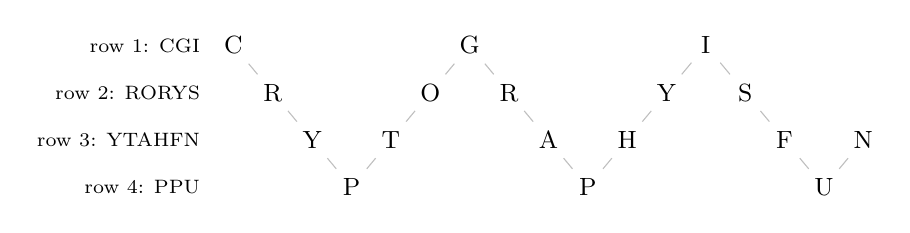
\begin{tikzpicture}
  \railfence{C/0,R/1,Y/2,P/3,T/2,O/1,G/0,R/1,A/2,P/3,H/2,Y/1,I/0,S/1,F/2,U/3,N/2}
  \foreach \i in {1,...,16}{\pgfmathtruncatemacro{\j}{\i+1}\draw[gray!50] (rf\i) -- (rf\j);}
  \node[font=\scriptsize,anchor=east] at (0.2,0) {row 1: CGI};
  \node[font=\scriptsize,anchor=east] at (0.2,-0.6) {row 2: RORYS};
  \node[font=\scriptsize,anchor=east] at (0.2,-1.2) {row 3: YTAHFN};
  \node[font=\scriptsize,anchor=east] at (0.2,-1.8) {row 4: PPU};
\end{tikzpicture}
\end{center}
Read along the line: \textbf{cryptographyisfun} (``cryptography is fun''). The same steps, with row counts 5, 10, 5, turn the homework answer above back into \ttx{nesoacademyisthebest}.

\begin{trap}[: unequal rows]
Do not assume the rows are equal, or that the middle rows are equal to each other. In Example 3 rows 2 and 3 have different lengths (5 and 6) because the message stops partway through a cycle, after the zig-zag has passed row 3 on its way up but before it reaches row 2.
\end{trap}

\subsection{Row--column transposition}
The rail fence has too few keys to be of any use. A more complex scheme uses a \textbf{rectangle}: the message is \textbf{written row by row} into a rectangle of $c$ columns and \textbf{read column by column}, but the columns are read in a \textbf{secret order}. The \textbf{key} is that order of the columns, written as a number above each column (the column marked 1 is read first). Leftover cells in the last row are filled with agreed filler letters (\ttx{x}, \ttx{y}, \ttx{z}), so that every column has the same height and the receiver can remove the fillers after decryption.

\textbf{Example:} ``Kill Corona Virus at twelve am tomorrow'' (33 letters), 7 columns $\times$ 5 rows = 35 cells, so 2 fillers (\ttx{y}, \ttx{z}). Key \textbf{4 3 1 2 5 6 7}.
\begin{center}\small
\begin{minipage}[c]{0.4\textwidth}\centering
\begin{tabular}{|*{7}{c|}}
\multicolumn{1}{c}{4}&\multicolumn{1}{c}{3}&\multicolumn{1}{c}{\textbf{1}}&\multicolumn{1}{c}{2}&\multicolumn{1}{c}{5}&\multicolumn{1}{c}{6}&\multicolumn{1}{c}{7}\\
\hline
k&i&\cellcolor{warn!18}l&l&c&o&r\\ \hline
o&n&\cellcolor{warn!18}a&v&i&r&u\\ \hline
s&a&\cellcolor{warn!18}t&t&w&e&l\\ \hline
v&e&\cellcolor{warn!18}a&m&t&o&m\\ \hline
o&r&\cellcolor{warn!18}r&o&w&\textit{y}&\textit{z}\\ \hline
\end{tabular}\\[2pt]
{\footnotesize numbers above = read order}
\end{minipage}
\begin{minipage}[c]{0.5\textwidth}
\begin{tabular}{@{}lll@{}}
\toprule
Order & Column & Letters\\
\midrule
1 & col 3 & LATAR\\
2 & col 4 & LVTMO\\
3 & col 2 & INAER\\
4 & col 1 & KOSVO\\
5 & col 5 & CIWTW\\
6 & col 6 & OREOY\\
7 & col 7 & RULMZ\\
\bottomrule
\end{tabular}
\end{minipage}
\end{center}
Answer: \textbf{\ttx{LATARLVTMOINAERKOSVOCIWTWOREOYRULMZ}}

\textbf{Key space and weakness.} With $c$ columns there are $c!$ reading orders ($7! = 5040$ here), multiplied by the choice of $c$, so brute force by hand is already tedious. The weakness is structural. Consecutive ciphertext letters come from one column, i.e.\ from plaintext positions exactly $c$ apart: the first five ciphertext letters are plaintext letters 3, 10, 17, 24, 31. An attacker who guesses the number of rows (here 5, a divisor of 35) cuts the ciphertext into 5-letter pieces, stands them side by side as columns and rearranges the columns until the rows read as English, guided by common digrams; Forouzan calls this the \textbf{pattern attack} (\S\ref{sec:classextra}). This is why the lecture says a single transposition ``can be reconstructed''.

\begin{worked}[: decrypting a row--column transposition]
\textbf{Q.} Decrypt \ttx{LATARLVTMOINAERKOSVOCIWTWOREOYRULMZ}, written row by row into 7 columns and read in the column order \textbf{4 3 1 2 5 6 7}.

\textbf{Column height.} $L = 35$ letters in 7 columns, so every column holds $35 / 7 = 5$ letters (5 rows).

\textbf{Refill the columns in key order.} The first 5 letters belong to the column numbered 1 (column 3), the next 5 to the column numbered 2 (column 4), and so on:
\begin{center}\small
\begin{tabular}{@{}llllllll@{}}
\toprule
Piece & LATAR & LVTMO & INAER & KOSVO & CIWTW & OREOY & RULMZ\\
Goes to column & 3 & 4 & 2 & 1 & 5 & 6 & 7\\
\bottomrule
\end{tabular}
\end{center}
\textbf{Read row by row.} Column 1 is now \ttx{KOSVO}, column 2 \ttx{INAER}, column 3 \ttx{LATAR}, and so on; reading the rebuilt grid across its rows gives \ttx{killcor | onaviru | sattwel | veamtom | orrowyz}. Removing the fillers \ttx{yz}, the plaintext is \textbf{kill corona virus at twelve am tomorrow}. Check: re-encrypting gives the received ciphertext \checkmark.
\end{worked}

\subsection{Two stages: more complex}
A single transposition leaves the regular pattern just described. The remedy is to \textbf{feed the ciphertext back in} and transpose again, usually with the same key:
\begin{center}\small
\begin{minipage}[c]{0.4\textwidth}\centering
\begin{tabular}{|*{7}{c|}}
\multicolumn{1}{c}{4}&\multicolumn{1}{c}{3}&\multicolumn{1}{c}{\textbf{1}}&\multicolumn{1}{c}{2}&\multicolumn{1}{c}{5}&\multicolumn{1}{c}{6}&\multicolumn{1}{c}{7}\\
\hline
L&A&\cellcolor{warn!18}T&A&R&L&V\\ \hline
T&M&\cellcolor{warn!18}O&I&N&A&E\\ \hline
R&K&\cellcolor{warn!18}O&S&V&O&C\\ \hline
I&W&\cellcolor{warn!18}T&W&O&R&E\\ \hline
O&Y&\cellcolor{warn!18}R&U&L&M&Z\\ \hline
\end{tabular}
\end{minipage}
\begin{minipage}[c]{0.5\textwidth}
Read columns 3, 4, 2, 1, 5, 6, 7:\\[2pt]
\ttx{TOOTR AISWU AMKWY LTRIO RNVOL LAORM VECEZ}
\end{minipage}
\end{center}
Answer: \textbf{\ttx{TOOTRAISWUAMKWYLTRIORNVOLLAORMVECEZ}}.
The full key is now: the rectangle size, the column order and the number of stages. To decrypt, the receiver applies the single-stage decryption of the worked example twice (the second stage is undone first).

\textbf{Why two stages are stronger.} After one stage, ciphertext positions 1--5 hold plaintext letters $3, 10, 17, 24, 31$: a run with constant step 7. After two stages they hold plaintext letters $17, 32, 8, 26, 7$ (computed by composing the two permutations), and no constant step appears anywhere in the ciphertext. Cutting the ciphertext into columns therefore no longer produces fragments of plaintext rows, and the attacker must undo both permutations at once instead of one rectangle at a time. Two stages are still a single permutation of the 35 positions (so the letter frequencies are still those of English), but it is not a \emph{columnar} permutation: it lies outside the small, regular family that the pattern attack searches. \S\ref{sec:classextra} repeats this analysis on Forouzan's keyed columnar example.

\begin{fixbox}
\begin{itemize}
  \item ``Thank you very much'', depth 3, is \ttx{TKVMHNYUEYUH}\textbf{\ttx{AORC}}. The notes' final string ends in \ttx{AORE}, but their own row reading gives \ttx{AORC}.
  \item Row--column: the speaker says ``R U L M C'' for column 7, but the grid (and slide) give \ttx{RULMZ}. All other results were checked by script and are correct.
  \item The OTP formulas, Shannon and $P(M\mid C) = P(M)$ come from Gemini's notes, not the slides. They are standard and correct.
\end{itemize}
\end{fixbox}
